%%%%%%%%%%%%%%%%%%%%%%%%%%%%%%%%%%%%%%%%%%%%%%%%%%%%%%%%%%%%%%%%%%%%%%%%%%%%%%%%%%%%%%%
%%%%%%%%%%%%%%%%%%%%%%%%%%%%%%%%%%%%%%%%%%%%%%%%%%%%%%%%%%%%%%%%%%%%%%%%%%%%%%%%%%%%%%%
% 
% This top part of the document is called the 'preamble'.  Modify it with caution!
%
% The real document starts below where it says 'The main document starts here'.

\documentclass[12pt]{article}
\usepackage{graphicx}
\usepackage{float}
\usepackage{amssymb,amsmath,amsthm}
\usepackage[top=1in, bottom=1in, left=1.25in, right=1.25in]{geometry}
\usepackage{fancyhdr}
\usepackage{enumerate}
\usepackage{listings}
\usepackage{verbatim}


% Comment the following line to use TeX's default font of Computer Modern.
\usepackage{times,txfonts}

\newtheoremstyle{homework}% name of the style to be used
  {18pt}% measure of space to leave above the theorem. E.g.: 3pt
  {12pt}% measure of space to leave below the theorem. E.g.: 3pt
  {}% name of font to use in the body of the theorem
  {}% measure of space to indent
  {\bfseries}% name of head font
  {:}% punctuation between head and body
  {2ex}% space after theorem head; " " = normal interword space
  {}% Manually specify head
\theoremstyle{homework} 

% Set up an Exercise environment and a Solution label.
\newtheorem*{exercisecore}{Exercise \@currentlabel}
\newenvironment{exercise}[1]
{\def\@currentlabel{#1}\exercisecore}
{\endexercisecore}

\newcommand{\localhead}[1]{\par\smallskip\noindent\textbf{#1}\nobreak\\}%
\newcommand\solution{\localhead{Solution:}}

%%%%%%%%%%%%%%%%%%%%%%%%%%%%%%%%%%%%%%%%%%%%%%%%%%%%%%%%%%%%%%%%%%%%%%%%
%
% Stuff for getting the name/document date/title across the header
\makeatletter
\RequirePackage{fancyhdr}
\pagestyle{fancy}
\fancyfoot[C]{\ifnum \value{page} > 1\relax\thepage\fi}
\fancyhead[L]{\ifx\@doclabel\@empty\else\@doclabel\fi}
\fancyhead[C]{\ifx\@docdate\@empty\else\@docdate\fi}
\fancyhead[R]{\ifx\@docauthor\@empty\else\@docauthor\fi}
\headheight 15pt

\def\doclabel#1{\gdef\@doclabel{#1}}
\doclabel{Use {\tt\textbackslash doclabel\{MY LABEL\}}.}
\def\docdate#1{\gdef\@docdate{#1}}
\docdate{Use {\tt\textbackslash docdate\{MY DATE\}}.}
\def\docauthor#1{\gdef\@docauthor{#1}}
\docauthor{Use {\tt\textbackslash docauthor\{MY NAME\}}.}
\makeatother

% Shortcuts for blackboard bold number sets (reals, integers, etc.)
\newcommand{\Reals}{\ensuremath{\mathbb R}}
\newcommand{\Nats}{\ensuremath{\mathbb N}}
\newcommand{\Ints}{\ensuremath{\mathbb Z}}
\newcommand{\Rats}{\ensuremath{\mathbb Q}}
\newcommand{\Cplx}{\ensuremath{\mathbb C}}
%% Some equivalents that some people may prefer.
\let\RR\Reals
\let\NN\Nats
\let\II\Ints
\let\CC\Cplx

%%%%%%%%%%%%%%%%%%%%%%%%%%%%%%%%%%%%%%%%%%%%%%%%%%%%%%%%%%%%%%%%%%%%%%%%%%%%%%%%%%%%%%%
%%%%%%%%%%%%%%%%%%%%%%%%%%%%%%%%%%%%%%%%%%%%%%%%%%%%%%%%%%%%%%%%%%%%%%%%%%%%%%%%%%%%%%%
% 
% The main document start here.

% The following commands set up the material that appears in the header.
\doclabel{Stat 300: Homework 3}
\docauthor{Stefano Fochesatto}
\docdate{\today}

\begin{document}

\textbf{2.56:} For any events $A$ and $B$ with $P(B) > 0$, show that $P(A|B) + P(A'|B) = 1$\\

\textbf{Solution:} Using the multiplication rule and set theory,
\begin{align*}
  P(A|B) + P(A'|B) &= \dfrac{P(A \cap B)}{P(B)} + \dfrac{P(A' \cap B)}{P(B)},\\
  &= \dfrac{P(A \cap B) + P(A' \cap B)}{P(B)},\\
  &= \dfrac{P(B)}{P(B)},\\
  &= 1. 
\end{align*}
Thus we hve show that for any events $A$ and $B$ where $P(B) > 0$ then $P(A|B) + P(A'|B) = 1$.
\vspace{1in}







\textbf{2.74:} Tho proportions of blood phenotypes in the U.S population are as follows:
 \begin{center}
\begin{tabular}{ c c c c}
  $A$ & $B$ & $AB$ & $O$ \\
  .40 & .11 & .04 & .45 \\
\end{tabular}
\end{center}
Assuming the phenotypes of two randomly selected individuals are independent of one another, what is the probability that both
phenotypes are $O$? what is the probability that the phenotype of two randomly selected individuals match.\\

\textbf{Solution:} Since the two randomly selected individuals are independent of each other we can simply use the multiplication rule to compute the
probability where both are type $O$,
\begin{equation*}
  P(O\cap O) = P(O)P(O) = .45^2 = .2025.
\end{equation*}
Furthermore we can calculate the probability that the phenotype of two randomly selected individuals match by performing the same operation and summing over each disjoint pair,
\begin{align*}
  P((O\cap O) \cup (A\cap A) \cup (B\cap B) \cup (AB\cap AB)) &= .45^2 + .40^2 + .11^2 +.04^2,\\
  &= .3762.
\end{align*}
\vspace{1in}













\textbf{2.78:} A boiler has five identical relief valves. The probability that any particular valve will open on demand is $.96$.
Assuming independent operation of the valves, calculate the probability that at least one valve opens and the probability that at least one valve fails to open.\\ 

\textbf{Solution:} First note that the probability that at least one valve opens is the same as the compliment of the probability that all valves fail. So since each valve is identical and independent,
\begin{equation*}
  P(\text{one valve opens}) = 1 - P(\text{all valves fail}) = 1 - .04^5 \approx 1.
\end{equation*}
Similarly we can calculate the probability that at least one valve fails,
\begin{equation*}
  P(\text{one valve fails}) = 1 - P(\text{all valves open}) = 1 - .96^5 \approx .1846.
\end{equation*}
\vspace{1in}






\textbf{2.82:} Consider independently rolling two fair dice, one res and the other green. Let $A$ be the event that the red die shows 3 dots, 
$B$ be the event that the green die shows 4 dots, and $C$ be the event that the total number of dots showing on the dice is 7. Are these events pairwise independent?\\

\textbf{Solution:} Recall, that to show two events $A$ and $B$ are independent we must demonstrate $P(A\cup B) = P(A)P(B)$. First we must calculate the sole
probabilities of $A, B$ and $C$. Note that the total number of rolls possible from 2 dice is our sample space, thus $S = 6^2$. Observe that the number of rolls where one of the die are fixed is 6, and therefore,
\begin{equation*}
  P(A) = P(B) = \dfrac{6}{6^2} = \dfrac{1}{6}.
\end{equation*}
Note the number of integer solutions to,
\begin{equation*}
  z_1 + z_2 = 7
\end{equation*}
where $1 \le z_{1,2} le 6$ is 6 and therefore,
\begin{equation*}
  P(6) = \dfrac{6}{6^2} = \dfrac{1}{6}.
\end{equation*}
Also note that any pairwise intersection of $A,B,C$ gives the roll $(3,4)$ in some form thus
\begin{equation*}
  P(A\cap B) = P(A\cap C) = P(C\cap B) =  \dfrac{1}{6^2}.
\end{equation*}
Since $P(A) = P(B) = P(C) = \frac{1}{6}$ we know that any pairwise multiplication of the probabilities will always yield $\frac{1}{6^2}$ thus the events are pairwise independent. 
\vspace{1in}


\textbf{2.88:} The probability that an individual randomly selected from a particular population had a certain disease is $.05$.
A diagnostic test correctly detects the presence of the disease $98\%$ of the time and correctly detects the absence of the disease $99\%$
of the time. If the test is applied twice, independently and return positive, what is the posterior probability that the selected individual had the disease?\\

\textbf{Solution:} First let event $A$ be that an individual has a disease, and let $B$ be the event where an individual tests positive. Using our terms recall what we were given,
\begin{align*}
  P(A) &= .05\\
  P(A') &= 1 - .05 = .95\\
  P(B|A) &= .98\\
  P(B|A') &= .99
\end{align*}
We want to find the probability that an individual has the disease given that they tested positive twice in two independent tests. Through Bayes' Rule we know that
\begin{equation*}
  P(A|BB) = \dfrac{P(BB\cap A)}{P(BB\cap A)+P(BB\cap A')}
\end{equation*} 
Because the tests are independent, by the multiplication rule we know that,
\begin{align*}
  P(BB\cap A) &= P(B \cap A)^2,\\
  &= (P(A)P(B|A))^2,\\
  &=.002401.
\end{align*}
Making the same argument for the  $P(BB\cap A')$ term, 
\begin{align*}
  P(BB\cap A) &= P(B \cap A')^2,\\
  &= (P(A')P(B|A'))^2,\\
  &=.00009025.
\end{align*}
Thus we find that the posterior probability is
\begin{equation*}
  P(A|BB) =\dfrac{P(BB\cap A)}{P(BB\cap A)+P(BB\cap A')} = \dfrac{.002401}{.002401 + .00009025} =.9638
\end{equation*}
\vspace{1in}




\textbf{3.2:} Give three example of bernoulli random variables?\\

\textbf{Solution:} Consider the following,
\begin{enumerate}
  \item The event that the next digit in a binary sequence is a 1.
  \item The event that the next digit in a natural number sequence has even parity.
  \item The event that the next digit in an integer number sequence, excluding zero is negative.
\end{enumerate}
\vspace{1in}







\textbf{3.12:} Airlines sometimes overbook flights. Suppose that for a plane of 50 seats, 55 passengers have a ticket. Define the random variables $Y$
as the number of ticketed passengers who actually show up for the flight. The Probability Mass Function (p(x)) is given.
\begin{enumerate}
  \item[\textbf{a.}] What is the probability that the flight will accommodate all the ticketed passengers who show up?\\
  
  \textbf{Solution:} Since the plane can only accommodate 50 people, all we hve to so is calculate $P(Y \le 50)$,
  \begin{equation*}
    P(Y \le 50) = \sum_{i = 45}^{50} p(i) = .83
  \end{equation*}
  \vspace{.25in}

  \item[\textbf{b.}] What is the probability that not all ticketed passengers who show up can be accommodated?\\
  
  \textbf{Solution:}Again since the plane can only accommodate 50 people we simply calculate $P(Y>50)$,
  \begin{equation*}
    P(Y > 50) = 1 - P(Y \le 50) = 1 - .83 = .17.
  \end{equation*}
  \vspace{.25in}

  \item[\textbf{c.}] If you are the first person in the standby list what is the probability that you will be able to board the flight? what is the
  probability in you are the third person on the list.\\

  \textbf{Solution:} Saying first person on standby to get a seat on the plane, is equivalent to at most 49 people showed up to the flight. Thus the probability that the 
  first standby person get on the plane is $P(Y \le 49)$,
  \begin{equation*}
    P(Y \le 49) = \sum_{i = 45}^{49} p(i) = .66.
  \end{equation*}
  Likewise for the third person on standby to get on the plane at most 47 people can show up. Thus the probability that third person on standby boards the plane is $P(Y \le 47)$,
  \begin{equation*}
    P(Y \le 47) = \sum_{i = 45}^{47} p(i) = .27.
  \end{equation*}
\end{enumerate}








\textbf{3.14:} A contractor is is required by the county planning department to submit one, two, three, four, and five forms in applying for a building permit.
Let $Y =$ the number of forms required of the next applicant the probability that $y$ are required is known to be proportional to $y$ - that is $p(y) = ky$ for $y \in [5]$.\\
\begin{enumerate}
  \item[\textbf{a.}] What is the value of $k$?\\
   
  \textbf{Solution:}Recall that the sum of a probability mass function over the support must sum to 1, and therefore we get,
  \begin{align*}
    1 &= \sum_{i = 1}^5 p(i),\\ 
    1 &= k(1+2+3+4+5),\\ 
    1&= k15,\\
    k &= \dfrac{1}{15}. 
  \end{align*}
  \vspace{.5in}



  \item[\textbf{b.}]What is the probability that at most three forms are required?\\
  
  \textbf{Solution:} Calculating $P(Y \le 3)$,
  \begin{equation*}
    P(Y \le 3) =  \sum_{i = 1}^3 p(i) = .4
  \end{equation*}
  \vspace{.5in}


  \item[\textbf{c.}] What is the probability that between 2 and 4 forms are required (inclusive)?\\
   
  \textbf{Solution:} Calculating $P(2 \le Y \le 4)$,
  \begin{equation*}
    P(2\le Y \le 4) =  \sum_{i = 2}^4 p(i) = .6
  \end{equation*}
  \vspace{.5in}


  \item[\textbf{d.}] Could $p(y) = \dfrac{y^2}{50}$ for  $y \in [5]$ be a pmf for $Y$\\
   
  \textbf{Solution:} Recall that by definition the values of a probability mass function must sum to one over the support of the random variable,
  \begin{equation*}
    \sum_{i = 1}^5 p(i) = \dfrac{1+4+9+16+25}{50} = 1.
  \end{equation*}
  Therefore $p(y)$ is a valid pmf for $Y$. 
\end{enumerate}





\textbf{3.18:} Two fair six-sided dice are tossed independently. Let $M = $ the maximum of the two tosses (so $M(1,5) = 5$).

\begin{enumerate}
  \item[\textbf{a.}] What is the pms of $M$?\\
 
  \textbf{Solution:} Note that for some value of a six sided dice, $i$ we have one pair where it shows up twice ie. $(i,i)$ and $2*(i-1)$ pairs where its is the largest of the pair ie. $(i,j)$ and $(j,i)$
  where $j < i$. Thus the proposed pmf for $M$ is,
  \begin{equation*}
    m(i) = \dfrac{2(i-1)}{36}
  \end{equation*}
  As an exercise we will prove its a valid pmf over the support $[6]$ using $r$,
  \textbf{Code:}
  \lstinputlisting{dice1.r}
  \textbf{Console:}
  \lstinputlisting{console}
  Thus $m$ is a valid pmf for $M$
  \vspace{.5in}

  \item[\textbf{b.}]Determine the cdf for $m$ and graph it.\\
  
  \textbf{Solution:}] By definition we know that the cdf for $m$ is simply, 
  \begin{equation*}
    m_c(x) = \sum_{i = 1}^x m(i) = \sum_{i = 1}^x \dfrac{2(i-1)}{36}
  \end{equation*} 
  Modifying our script from the previous problem we get, 
  \textbf{Code:}
  \lstinputlisting{dice.R}
  \textbf{Plot:}
  \begin{center}
    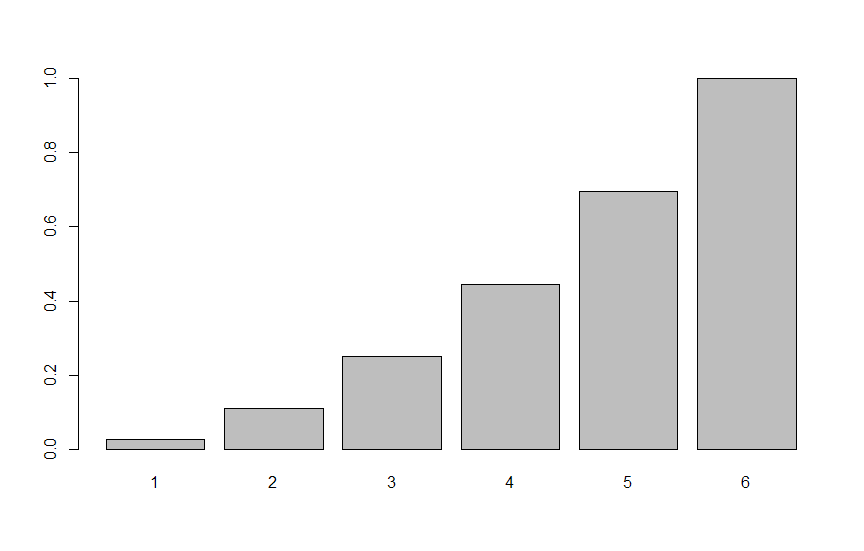
\includegraphics[width = .75\textwidth]{rplot.png}  
  \end{center}
  





\end{enumerate}






























































































































\vspace{1in}




























\end{document}